
\documentclass[tikz, border=10mm]{standalone}
\usepackage{xcolor}
\usepackage{tikz}
\usetikzlibrary{positioning, calc, backgrounds, quotes, arrows.meta}

% Color Definitions (Matching nn_blocks.tex)
\definecolor{ConvColor}{rgb}{0.98,0.81,0.69}
\definecolor{PoolColor}{rgb}{0.8,0.33,0.33}
\definecolor{UnpoolColor}{rgb}{0.6,0.7,0.9}
\definecolor{FcColor}{rgb}{0.6,0.2,0.8}
\definecolor{ResBlockColor}{rgb}{0.85,0.92,1.0}

% 2D Style (Flowchart)
\tikzset{
    layer/.style={
        rectangle,
        rounded corners=1mm,
        minimum height=2.0em,
        minimum width=3.0em,
        align=center,
        draw=black!80,
        thick
    },
    conv/.style={layer, fill=ConvColor},
    pool/.style={layer, fill=PoolColor},
    up/.style={layer, fill=UnpoolColor},
    res/.style={layer, fill=ResBlockColor},
    fc/.style={layer, fill=FcColor},
    skip/.style={->, dashed, draw=blue!60, thick}
}

\begin{document}
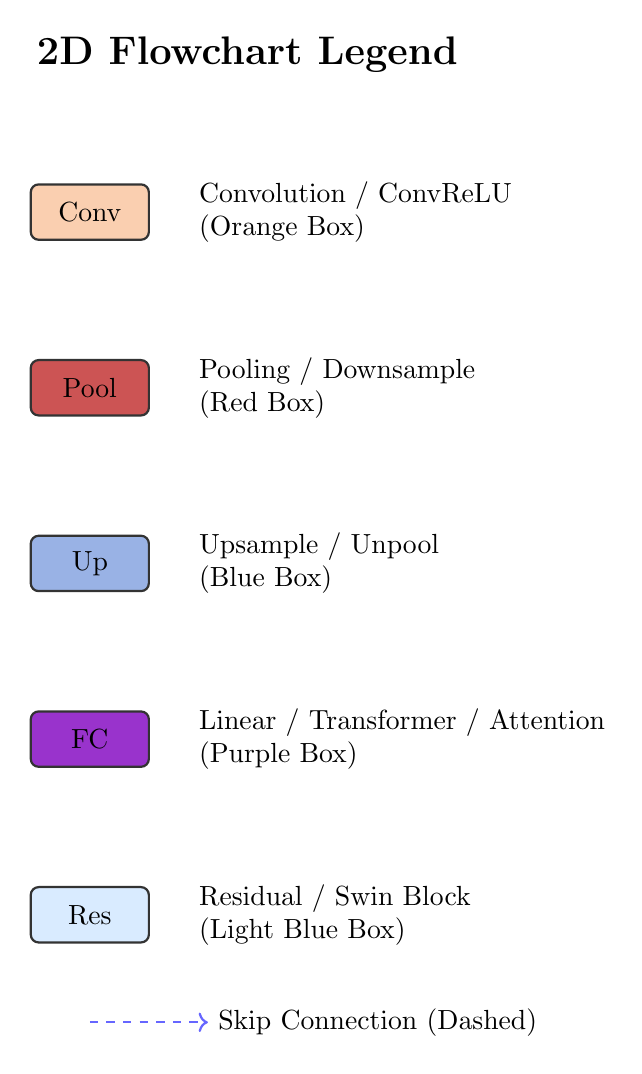
\begin{tikzpicture}[node distance=0.8cm, every node/.style={transform shape}]

% Title
\node[font=\Large\bfseries] at (2, 7) {2D Flowchart Legend};

\coordinate (start) at (0, 5);

% Conv
\node[conv, minimum width=1.5cm] (n_conv) at (start) {Conv};
\node[right=0.5cm of n_conv, align=left] {Convolution / ConvReLU\\(Orange Box)};

% Pool
\node[pool, minimum width=1.5cm, below=1.5cm of n_conv] (n_pool) {Pool};
\node[right=0.5cm of n_pool, align=left] {Pooling / Downsample\\(Red Box)};

% Up
\node[up, minimum width=1.5cm, below=1.5cm of n_pool] (n_up) {Up};
\node[right=0.5cm of n_up, align=left] {Upsample / Unpool\\(Blue Box)};

% FC
\node[fc, minimum width=1.5cm, below=1.5cm of n_up] (n_fc) {FC};
\node[right=0.5cm of n_fc, align=left] {Linear / Transformer / Attention\\(Purple Box)};

% Res
\node[res, minimum width=1.5cm, below=1.5cm of n_fc] (n_res) {Res};
\node[right=0.5cm of n_res, align=left] {Residual / Swin Block\\(Light Blue Box)};

% Skip
\draw[skip] ($(n_res.south) + (0, -1)$) -- ++(1.5, 0) node[right] {Skip Connection (Dashed)};

\end{tikzpicture}
\end{document}
